\documentclass[letterpaper,10pt]{article}

\usepackage{titling}
\usepackage{listings}
\usepackage{url}
\usepackage{setspace}
\usepackage{subfig}
\usepackage{sectsty}
\usepackage{pdfpages}
\usepackage{colortbl}
\usepackage{multirow}
\usepackage{relsize}
\usepackage{amsmath}
\usepackage{fancyvrb}
\usepackage{amsmath,amssymb,amsthm,graphicx,xspace}
\usepackage[titlenotnumbered,noend,noline]{algorithm2e}
\usepackage[compact]{titlesec}
\usepackage{paratype} 
\usepackage[T1]{fontenc}
\usepackage{tikz}
\usetikzlibrary{arrows,automata,shapes,trees,matrix,chains,scopes,positioning,calc}
\tikzstyle{block} = [rectangle, draw, fill=blue!20, 
    text width=2.5em, text centered, rounded corners, minimum height=2em]
\tikzstyle{bw} = [rectangle, draw, fill=blue!20, 
    text width=4em, text centered, rounded corners, minimum height=2em]

\definecolor{namerow}{cmyk}{.40,.40,.40,.40}
\definecolor{namecol}{cmyk}{.40,.40,.40,.40}

\let\LaTeXtitle\title
\renewcommand{\title}[1]{\LaTeXtitle{\textsf{#1}}}


\newcommand{\handout}[5]{
  \noindent
  \begin{center}
  \framebox{
    \vbox{
      \hbox to 5.78in { {\bf ECE254: Operating Systems and Systems Programming } \hfill #2 }
      \vspace{4mm}
      \hbox to 5.78in { {\Large \hfill #4  \hfill} }
      \vspace{2mm}
      \hbox to 5.78in { {\em #3 \hfill} }
    }
  }
  \end{center}
  \vspace*{4mm}
}

\newcommand{\lecture}[3]{\handout{#1}{#2}{#3}{Lecture #1}}
\newcommand{\tuple}[1]{\ensuremath{\left\langle #1 \right\rangle}\xspace}

\addtolength{\oddsidemargin}{-1.000in}
\addtolength{\evensidemargin}{-0.500in}
\addtolength{\textwidth}{2.0in}
\addtolength{\topmargin}{-1.000in}
\addtolength{\textheight}{1.75in}
\addtolength{\parskip}{\baselineskip}
\setlength{\parindent}{0in}
\renewcommand{\baselinestretch}{1.5}
\newcommand{\term}{Spring 2015}

\singlespace


\begin{document}

\lecture{ 3 --- Operating System Structure and Traps}{\term}{Jeff Zarnett}

\section*{Operating System Structure}

An operating system is large and complex and this is not the sort of thing programmers create at a whim with no planning. It is possible to write an OS without a defined structure, but just like writing any large program, it will quickly become unmaintainable and will very likely be bug-riddled. Consider the traditional UNIX structure:

\begin{center}
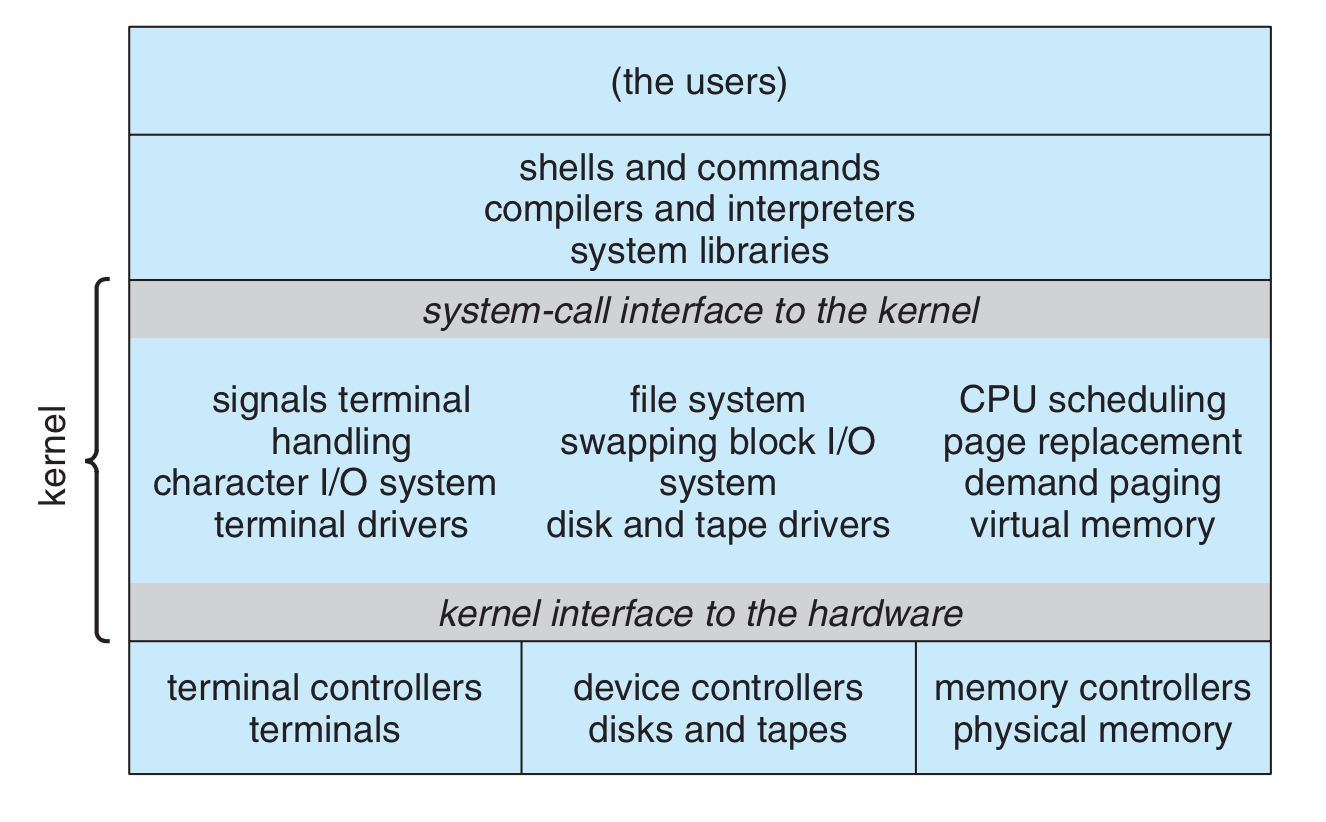
\includegraphics[width=0.5\textwidth]{images/unix-structure.png}\\
The traditional UNIX structure\cite{osc}.
\end{center}

There are some clearly defined areas here and interfaces between the kernel and hardware and between the user space and the kernel. Let us generalize this concept to a ``layered'' operating system: 

\begin{center}
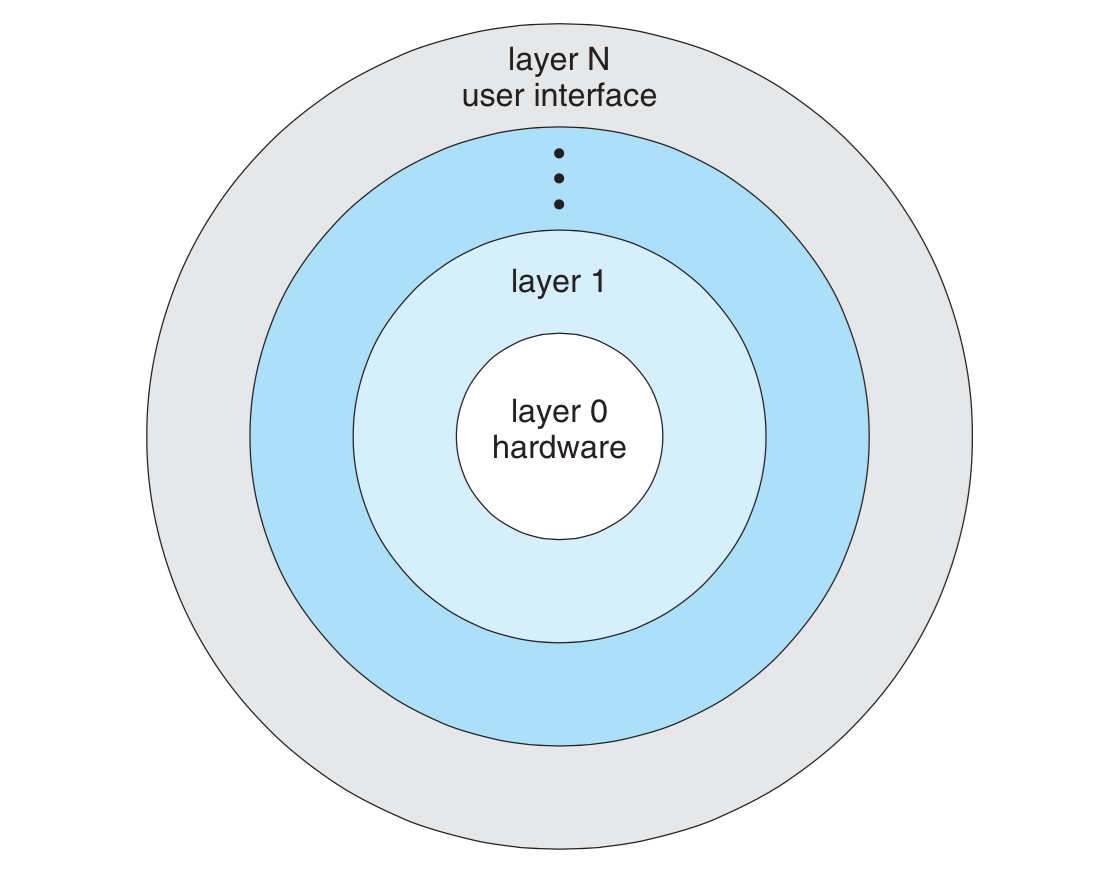
\includegraphics[width=0.5\textwidth]{images/layered-os.png}\\
A layered operating system~\cite{osc}.
\end{center}

All the modern desktop/laptop/mobile operating systems tend to follow this structure, with some modifications (the lines are not always so cleanly drawn). There is one further structural element that OSes have, within a layer: modules.

Just as we have classes and packages in a regular program to contain related functionality, an operating system's layers will have its functionality grouped into modules by what they do. We may have a module for a device driver, for scheduling, and for a file system.

Modules might be static, but more often they are loadable and swappable. So at run-time, or perhaps a reboot, we can replace a module with another version or add a new module. When connecting a new device to the system, if the device driver for it is not already loaded into the kernel, it can be done dynamically. As another example, we might choose to change scheduling from high responsiveness to high CPU usage, and this will require a reboot but not recompiling and reinstalling the kernel. The diagram below shows the loadable modules of Sun Microsystems' Solaris operating system:

\begin{center}
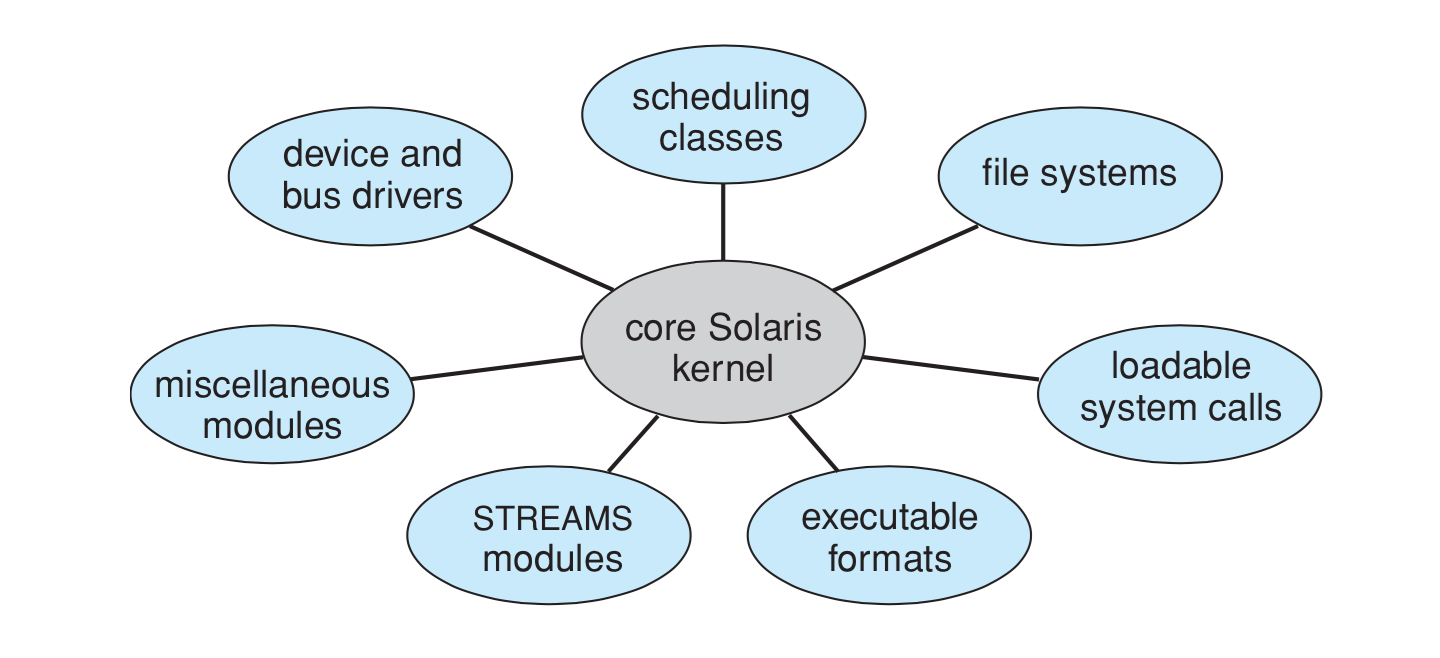
\includegraphics[width=0.65\textwidth]{images/solaris-structure.png}\\
Solaris loadable modules~\cite{osc}.
\end{center}

Combining the layered and modular approaches presents us with: the layered operating system with modules (not a very exciting name, I realize).

\subsection*{The Layered Operating System with Modules}

The operating system provides the environment for the execution of programs and supports them in their execution by providing various services. Some of the services are there for the convenience of the user programs; others are mandatory (e.g., to request memory, the user program MUST request it and can't simply take it). Consider the diagram below, which identifies some common categories of OS services and their relation to one another.

\begin{center}
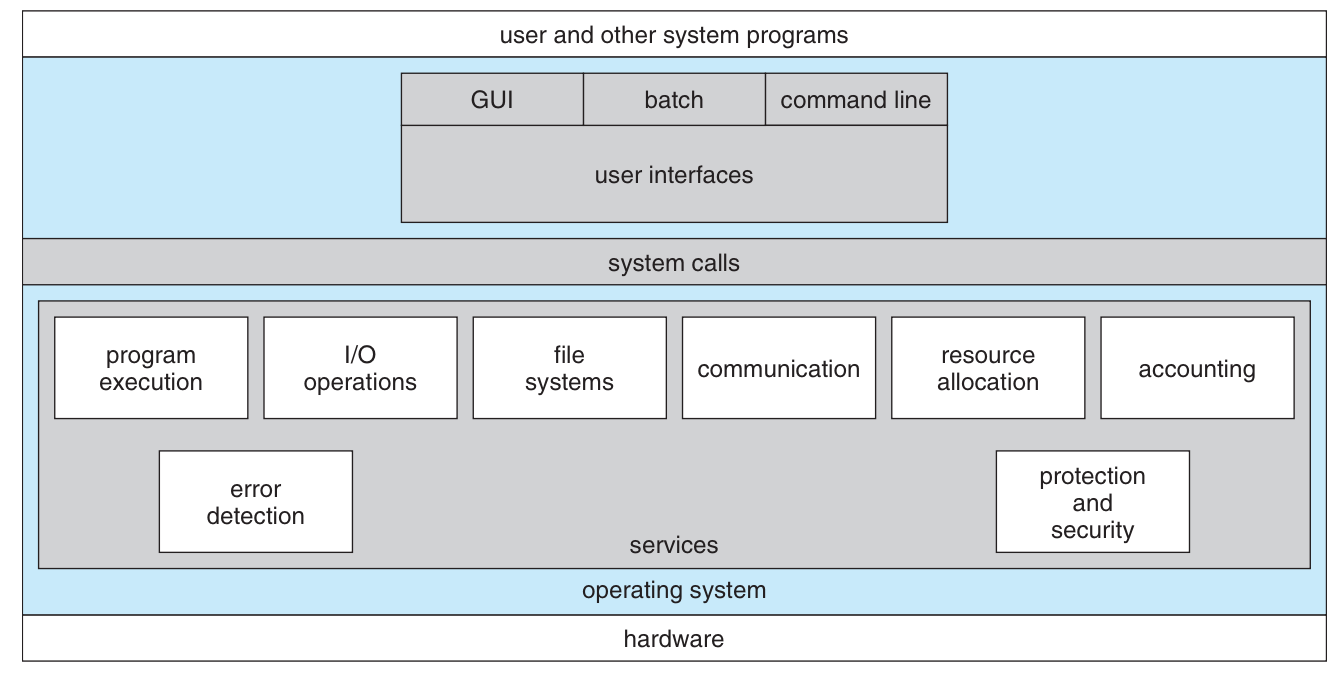
\includegraphics[width=0.75\textwidth]{images/os-structure.png}\\
A view of operating system services~\cite{osc}.
\end{center}

Let us take a moment to get an overview of these services, starting at the top and working our way down. Many of these services are something we will examine in detail later on.

\paragraph{The User Interface.} In the diagram the user interface is a box with several constituent parts: the GUI (Graphical User Interface, i.e., windows), the batch interface (commands entered in files that run periodically), and the command line interface (CLI). This is how the user (or a program) executes a program or command and how the results of that command are returned to the user.

\paragraph{System Calls.} System calls are functions or procedures the operating system makes available for use. It is the gateway into the operating system's functionality. When a user program wants to do something it cannot do itself, it makes a system call and that system call activates a portion of the OS functionality in the layer below.

\paragraph{Program Execution.} This is nothing more than the ability to load a program into memory and run it, as well as terminate the program (normally or otherwise)~\cite{osc}.

\paragraph{I/O Operations.} The operating system typically manages the I/O devices of the system, like printers, sensors, and actuators. We will examine shortly why the OS is the designated manager for this. When a new device is connected, like a USB key being plugged in, the OS needs to recognize it, initialize it, and make it available.

\paragraph{File Systems.} Files are important parts of the system -- they are programs and data. A program will need to read and write files, and the operating system does the same (such as when loading a program into memory to execute it). The file system is somewhat like the intersection of memory and an I/O device; the operating system manages both of those, so it is obvious it should also manage the file system.

\paragraph{Communication.} This may be communication between the computer and the Internet or between multiple processes in the same system. There are two basic strategies, each of which we will examine in due course: shared memory (in the same system) and message passing.

\paragraph{Resource Allocation.} In a system with multiple users or multiple programs, resources like memory need to be managed appropriately. Resources are limited even if there is enough to go around: two programs can't use the same area of memory at the same time. The OS is responsible for allocation of those resources, keeping track of which programs currently own a resource, and mediating conflicting requests.

\paragraph{Accounting.} It is usually desirable to keep some statistical data on what resources programs are using. This might be to ensure stability, as a way of improving usage, or just for billing. A program that is consuming too much memory or CPU may be terminated to ensure the system's stability. The data collected can be analyzed to find bottlenecks in the system that might be relieved. Or, in the case of something like a supercomputer, perhaps the operators will bill the users (typically universities and government departments) for how much of the CPU time they have used.

\paragraph{Error Detection.} The OS will need to detect and handle errors. Errors might come from user programs (like a division by zero) or from I/O devices (scanner has crashed). When the OS detects an error it may result in halting the system (the famous ``Blue Screen of Death'') or killing the offending program (``Would you like to report the problem to Microsoft?'')

\paragraph{Protection and Security.} The security side of this includes authentication (logging in to the system) and enforcing access rights on elements of the system (user vs. administrator accounts or who can read a file). Protection is about making sure all users and programs get along (as best they can): that one program doesn't interfere with the execution of another.


\paragraph{Invoking System Calls}
Some of the operating system services, like the accounting routines, run automatically and user programs do not interact with them. The rest, however, a user program may wish to interact with them. How do we do so?

\section*{It's a Trap!}
Operating systems run, as previously discussed, on interrupts. In addition to the interrupts that will be generated by hardware and devices (e.g., a keyboard signalling that the F1 key has been pressed), there are also interrupts generated in software. These are often referred to as a \textit{trap} (or, sometimes, an exception). The trap is usually generated either by an error like an invalid instruction or from a user program request. 

If it is simply an error the operating system will decide how to deal with it, and in desktop/laptop OSes, the usual strategy is sending the exception to the program that caused it, and this is usually fatal to the offending program. Your programming experience will tell you that you can sometimes deal with an exception (perhaps through the language equivalent of the Java/C\# \texttt{try-catch-finally} syntax), but often an exception is unhandled and terminates the program.

The more interesting case is the intentional use of the trap: this is how a user program gets the operating system's attention. When a user program is running, the operating system is not; we might even say it is ``sleeping''. If the program running needs the operating system to do something, it needs to wake up the OS: interrupt its sleep. When the trap occurs, the interrupt handler (part of the OS) is going to run to deal with the request. 

Already we saw the concept of user mode vs. supervisor mode instructions: some instructions are not available in user mode. Supervisor mode, also called kernel mode, allows all instructions and operations. Even something seemingly simple like reading from disk or writing to console output requires privileged instructions. These are common operations, but they involve the operating system every time.

Modern processors keep track of what mode they are in with the mode bit. This was not the case for some older processors and some current processors have more than two modes, but we will restrict ourselves to dual-mode operation with a mode bit. Thus we can see at a glance which mode the system is in. At boot up, the computer starts up in kernel mode as the operating system is started and loaded. User programs are always started in user mode. When a trap or interrupt occurs, and the operating system takes over, the mode bit is set to kernel mode; when it is finished the system goes back to user mode before the user program resumes~\cite{osc}.

Suppose a text editor wants to output data to a printer. Management of I/O devices like printers is the job of the OS, so to send the data, the text editor must ask the OS to step in, as in the diagram below:

\begin{center}
	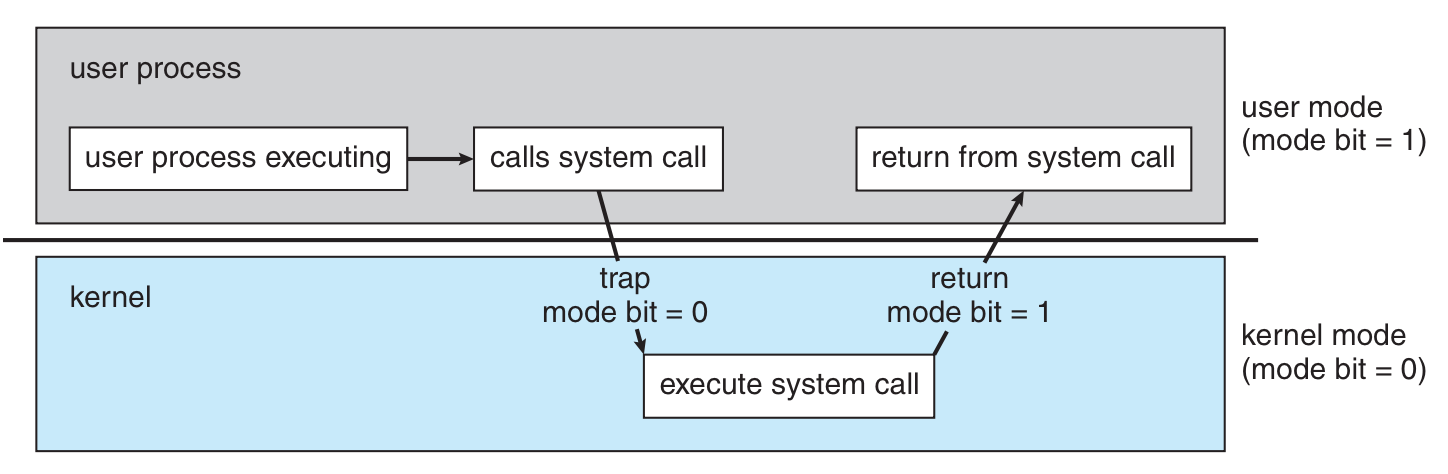
\includegraphics[width=0.75\textwidth]{images/trap.png}\\
	Transition from user to supervisor (kernel) mode~\cite{osc}.
\end{center}


So to print out the data, the program will prepare the data for printing. Then it calls the system call. You may think of this as being just like a normal function call, except it involves the operating system. This triggers the operating system (with a trap). The operating system responds and executes the system call and dispatches that data to the printer. When this job is done, operation goes back to user mode and the program returns from the system call.

\subsection*{Motivation for Dual Mode Operation}

Why do we have user and supervisor modes, anyway? As Uncle Ben told Spiderman, ``with great power comes great responsibility''. Many of the reasons are the same as why we have user accounts and administrator accounts: we want to protect the system and its integrity against errant and malicious users.

An example: multiple programs might be trying to use the same I/O device at once. If Program~1 tries to read from disk, it will take time for that request to be serviced. During that time, if Program~2 wants to read from the same disk, the operating system will force Program~2 to wait its turn. Without the OS to enforce this, it would be up to the author(s) of Program~2 to check if the disk is currently in use and to wait patiently for it to become available. That may work if everybody plays nicely, but without someone to enforce the rules, sooner or later there will be a program that does something nasty, like cancel another program's read request and perform its read first.

This doesn't come for free, of course: there is a definite performance trade-off. Switching from user mode to kernel mode requires some instructions and some time. It would be faster if everything ran in kernel mode because we would spend no time switching. Despite this, the performance hit for the mode switch is judged worthwhile for the security and integrity benefits it provides.

\subsection*{Example: Reading from Disk}
Let us examine in some more detail what is actually happening in a system call. This example is from~\cite{mos} and will use C code to perform a read on a UNIX system. The specification says the function \texttt{read} takes three parameters: (1) the file name; (2) where to read the data to; and (3) how many bytes to read. Here is an example: 

\begin{verbatim}
int bytesRead = read( filename, buffer, numBytes );
\end{verbatim}

(The \texttt{read} function returns the number of bytes successfully read; it is normally equal to \texttt{numBytes} but might be smaller if the end of the file is reached. Here we are storing it in a variable \texttt{bytesRead}.)

In preparation for invocation of \texttt{read} the parameters are pushed on the stack. This is the normal way in which a procedure is called in C(++). Then the \texttt{read} procedure is called and this is just the normal instruction to enter another function. The \texttt{read} function will put its identifier (the system call number) in a predefined location (typically a register). Then it executes the \texttt{trap} instruction, activating the OS.

When the \texttt{trap} occurs, the OS takes over and control switches from user mode to kernel mode. Control transfers to a predefined memory location within the kernel (the trap handler). The trap handler then runs and examines the request: it checks the identifier that was put in the register earlier. Based on that, it knows what system call request handler should execute: the one to read from a file. That routine executes. When it is finished, control will be returned to the \texttt{read} function; we exit the kernel and return to user mode.

Back in user mode, the \texttt{read} call finishes and returns, and control goes back to the user program.

\subsection*{Summary: Invoking a System Call}

To summarize, the steps, arranged chronologically, when invoking a system call are:
\begin{enumerate}
	\item The user program pushes arguments onto the stack.
	\item The user program invokes the system call.
	\item The system call puts its identifier in the designated location.
	\item The system call issues the \texttt{trap} instruction.
	\item The OS responds to the interrupt and examines the identifier in the designated location.
	\item The OS runs the system call handler that matches the identifier.
	\item When the handler is finished, control exits the kernel and goes back to the system call (in user mode).
	\item The system call returns control to the user program.

\end{enumerate}






\bibliographystyle{alpha}
\bibliography{254}


\end{document}